

\begin{frame}
	\frametitle{Cosmological N-body Simulations}
	
	\begin{itemize}
		\item N-body simulations are simulations of the motion of particles under the influence of physical forces.
		\item Focus on collisionless dark matter particles: 
		
		\begin{itemize}
			\item   hypothetical type of matter 
			\item 	the only significant interaction between the particles is via gravity
		\end{itemize}
	
	\end{itemize}
	
\end{frame}








\begin{frame}
	\frametitle{Cosmological N-body Simulations}
	
	\begin{itemize}
		\item After some time, the particles will clump together. Such gravitationally bound objects are called \emph{halos}.
		\item Halos themselves may contain self-bound objects, called \emph{subhalos}.
		\item The identification of halos and subhalos is an important tool for problems concerning cosmic structure and its formation.
		\item Codes that perform this task are called \emph{halo-finders}.
	\end{itemize}
	
\end{frame}














\begin{frame}
	\frametitle{Cosmological N-body Simulations}

	\begin{columns}
		\column{.25\textwidth}
			The results of a cosmological simulation of $128^3$ dark
			matter particles at redshift $z = 0$ with $H_0 = 70.4$ and density parameters $\Omega_m = 0.272$ and $\Omega_\Lambda= 0.728$.
			The box length corresponds to 88.8 Mpc.
			\vfill
		\column{.75\textwidth}
			\begin{figure}
				\centering
				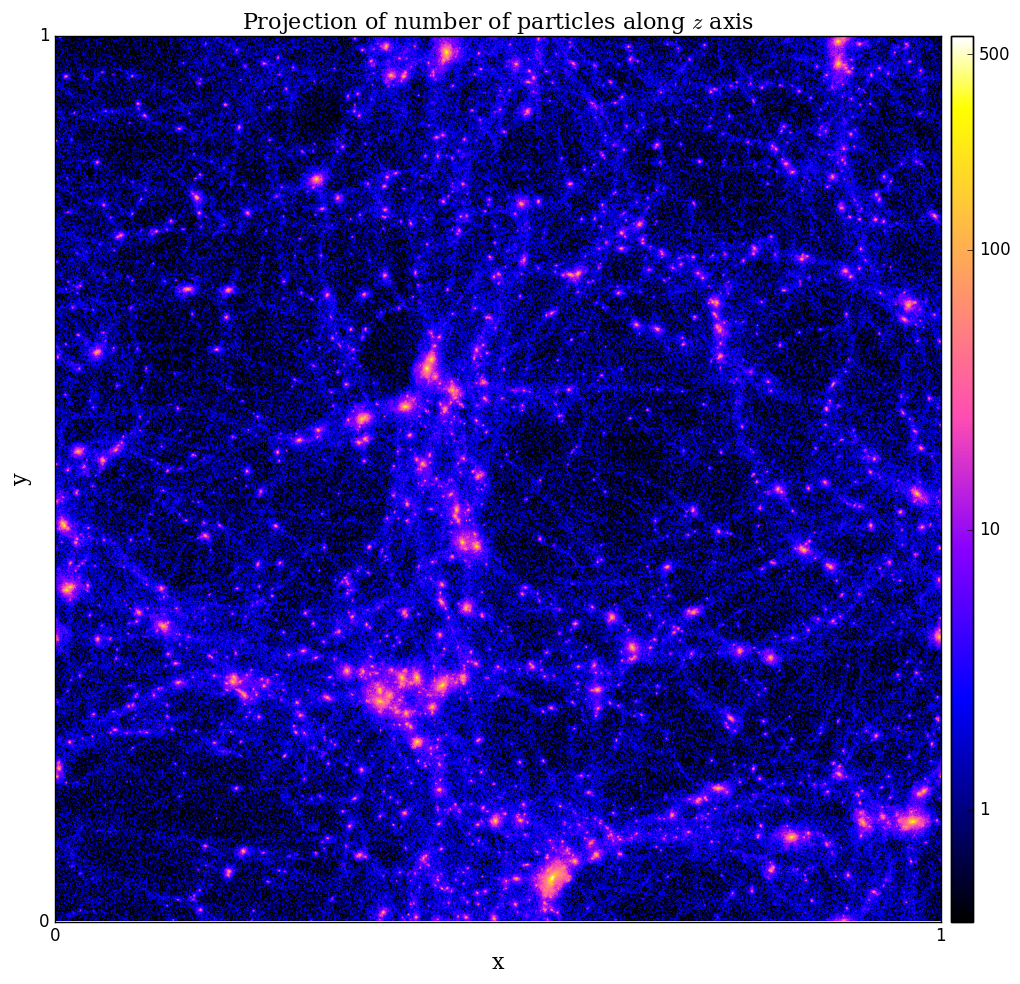
\includegraphics[width=8.2cm]{../report/images/cosmo/cos-part2map-npart.png}
		%		\caption{
		%		}
			\end{figure}
		\vfill
	\end{columns}

\end{frame}










\begin{frame}
	\frametitle{Unbinding Particles}


	\begin{itemize}
		\item By convention, it is customary to treat all particles assigned to a halo as bound to it, even though from a strict energetic perspective they may not be.
		\item For subhalos, on the other hand, it is vital to identify and remove unbound particles:
		\begin{itemize}
			\item Subhalos are located within a host halo and therefore expected to be contaminated by the host's particles
			\item Usually subhalos contain far less particles than their hosts, so assigning particles to it without an unbinding procedure can influence its physical properties significantly.
		\end{itemize}
		\item ``Removing a particle'' means here to assign it to the parent structure. This applies recursively to any level of substructure within substructure.
	\end{itemize}


\end{frame}







\begin{frame}
	\frametitle{Goals of this thesis}


	\begin{itemize}
		\item \ramses\ \parencite{ramses} is a N-body and hydrodynamical code that %
		contains a clump finding algorithm, \phew\ \parencite{PHEW}.
		%makes use of the adaptive mesh refinement technique: The entire computational domain is covered by cells, and smaller and smaller cells are introduced where necessary to achieve the desired accuracy.
%		\item \phew\ \parencite{PHEW} is a clump finding algorithm that can identify halos on-the-fly within the framework of \ramses.
		
		\item Both \phew\ and \ramses\ are fully parallel and make use of the MPI library. \phew\ works on-the-fly.
		
		\item The goal of this thesis is to implement a particle unbinding algorithm to work with \phew\ that is also fully parallel and works on-the-fly.
	\end{itemize}



\end{frame}








